\chapter{Perulangan (\textit{Looping})}

\section{Perulangan}
Seperti sudah dijelaskan Bab \ref{ch:konsepDasarAlgoritma} : ``Konsep Dasar Algoritma \& Pemrograman``, \textit{Repetition/Looping}(Perulangan) merupakan salah satu stuktur dasar algoritma. Pada algoritma, perulangan dipanggil dengan menggunakan \textit{statement} (\textit{for}) dan (\textit{while}). Masing - masing dari \textit{statement} ini memiliki cara kerjanya masing - masing sesuai yang telah dijelaskan pada beberapa sub-bab sebelumnya.   \\
\hfill \break
\textbf{Struktur perulangan secara umum terdiri atas dua bagian:}
\begin{enumerate}
	\item \textbf{Kondisi Perulangan}, yaitu ekspresi boolean yang harus dipenuhi untuk melaksanakan perulangan. Kondisi ini ada yang dinyatakan secara eksplisit maupun implisit
		\item \textbf{Badan Perulangan(body)}, yaitu bagian algoritma yang akan diulang ketika kondisi dipenuhi \\
\end{enumerate}
\hfill \break
\textbf{Struktur pengulangan biasanya disertai dengan bagian berikut:} 
\begin{enumerate}
	\item \textbf{Inisialisasi}, yaitu aksi yang dilakukan sebelum pengulangan dilakukan pertama kali 
	\item \textbf{Terminasi}, yaitu aksi yang dilakukan setelah pengulangan selesai dilaksanakan
\end{enumerate}
Inisialisasi dan terminasi tidak selalu arus ada, namun pada beberapa kasus (jika menggunakan \textit{while}), inisialiasi diperlukan. \\
\hfill \break
Bedasarkan peraturan diatas, struktur perulangan secara umum adalah sebagai berikut : 
\newpage
\begin{Petunjuk}
\label{Ptk:Struktur Perulangan}
	\textbf{Struktur Perulangan}\\
		\textit{inisialiasi}\\
		\textit{awal pengulangan}(dengan / atau tanpa kondisi)\\
		~~~~~\textit{badan pengulangan}\\
		\textit{akhir pengulangan}\\
		\textit{terminasi}\\
\end{Petunjuk}

%\textit{statement} \textit{for} digunakan untuk mengiterasi sebuah \textit{array}, \textit{list} ataupun kumpulan variabel/objek lainnya sedangkan \textit{statement} \textit{while} digunakan untuk perulangan yang berdasarkan kondisi tertentu.

\subsection{Perulangan dengan \textit{for}}
Konstruksi \textit{for} digunakan untuk menghasilkan pengulangan sejumlah kali yang telah diberitahukan sebelumnya. Jumlah pengulangan sudah diketahui atau dapat ditentukan sebelum eksekusi. Perulangan \textit{for} juga bisa ditentukan dimulai dari kapan, berhenti pada saat kapan, dan melangkah seberapa banyak dari mulai sampai akhir. \\

Untuk struktur \textit{while} bisa dilihat sebagai berikut : 
\begin{tabbing}

\textbf{for} $i$ \textbf{in} $x$:~~\=\ \\
~~~~~badan perulangan\\
\end{tabbing}
\textbf{atau}
\begin{tabbing}
\textbf{for} $i$ \textbf{in} range([start=0],stop,[step=1]):\\
~~~~~badan perulangan\\
\end{tabbing}


Contoh penggunaan format Python untuk iterasi isi dari List bisa dilihat di Listing \ref{lst:iterasiArray}.
\begin{listprog}{iterasiList.py}
	\label{lst:iterasiArray}
	\begin{lstlisting}[language=Python]
		A = [4,1,3,5]
		for i in A:
			print i
		#Hasil print berupa 4 1 3 5
	\end{lstlisting}
\end{listprog}

Sedangkan untuk mencetak rangkaian bilangan misalnya dari 1 sampai 10 bisa menggunakan fungsi \textit{range}. Contohnya bisa dilihat di Listing \ref{lst:cetakBilangan}
\begin{listprog}{cetakBilangan.py}
	\label{lst:cetakBilangan}
	\begin{lstlisting}[language=Python]
		for i in range(1,11):
			print i
		#Hasil print berupa 1 2 3 4 5 6 7 8 9 10
	\end{lstlisting}
\end{listprog}

\newpage

Untuk \textit{flowchart} \textit{for} bisa dilihat di Gambar \ref{fig:flowchartFor}.
\begin{marginfigure}[3cm]%
\centering
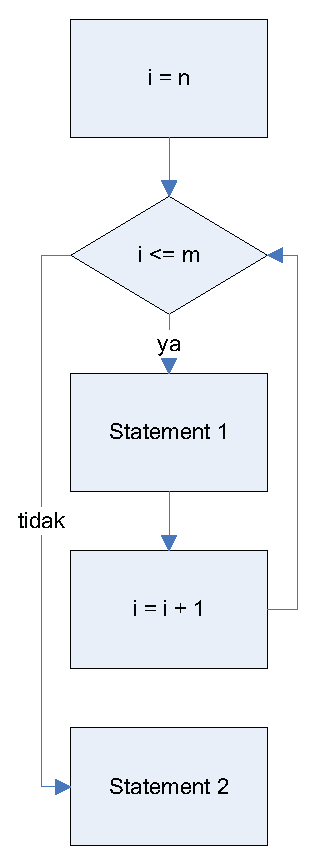
\includegraphics[scale=0.5]{fig/flowchart-FOR.eps}%
\caption{\Centering Notasi Algoritmik dengan Flowchart Untuk For}%
\label{fig:flowchartFor}%
\end{marginfigure}


\subsection{Perulangan dengan \textit{while}}
Konstruksi \textit{while} digunakan untuk menghasilkan pengulangan sejumlah kali selama kondisi ekspresi memenuhi. Badan perulangan pada \textit{while} akan dilaksanakan terus-menerus selama kondisi bernilai \textit{TRUE}. Jika kondisi sudah bernilai \textit{FALSE} maka badan perulangan tidak akan dimasuki dan pengulangan akan selesai.

\FloatBarrier
Untuk struktur \textit{while} bisa dilihat sebagai berikut.
\begin{tabbing}
\textbf{while} (Kondisi Logika):~~~~~~~~~~~~~~~\=\#Menjalankan perulangan selama kondisi benar\\
~~~~~\textit{statement}s\\
\end{tabbing}

Contoh penggunaan \textit{while} dalam bahasa Python untuk mencetak menurun bilang 10 sampai 1 bisa dilihat di Listing \ref{lst:cetakBilanganTurun}.
\begin{listprog}{cetakBilanganTurun.py}
	\label{lst:cetakBilanganTurun}
	\begin{lstlisting}[language=Python]
		i = 10
		while(i>0):
			print i
			i = i - 1	\end
		#Hasil print berupa 10 9 8 7 6 5 4 3 2 1
	\end{lstlisting}
\end{listprog}


Untuk \textit{flowchart} \textit{while} bisa dilihat di Gambar \ref{fig:flowchartWhile}.
\begin{marginfigure}[3cm]%
\centering
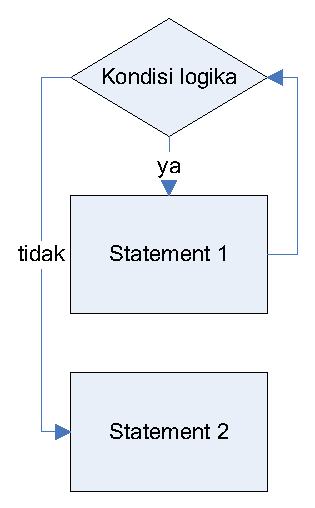
\includegraphics[scale=0.6]{fig/flowchart-WHILE.eps}%
\caption{\Centering Notasi Algoritmik dengan Flowchart Untuk While}%
\label{fig:flowchartWhile}%
\end{marginfigure}


\section{Implementasi Perulangan}
Pada sub-bab ini kita akan melihat bagaimana skenario - skenario penggunaan struktur pengulangan pada algoritma. Perulangan merupakan struktur dasar yang butuh waktu unuk dimengerti.Untuk mahir dalam pengulangan diperlukan banyak latihan dalam berbagai permasalahan yang melibatkan struktur perulangan.

Berikut ini adalah skenario - skenario dimana perulangan dibutuhkan : 
\begin{enumerate}
	\item Perulangan dibutuhkan bilamana kita ingin mengeksekusi perintah yang sama berkali-kali. Bayangkan pada keadaan dimana kita memerlukan pencetakan sebuah string sebanyak 10(Sepuluh) kali. Melakukan perintah sebanyak 10(Sepuluh) kali masih dapat di-manage dengan sequence(runtunan), tetapi bagaimana jika diminta 100.000(Seratus Ribu) kali. Tentunya ukuran kode sumber untuk algoritma akan membengkak seiring dengan jumlah perintah yang dilakukan. Perhatikan dua contoh berikut :
	
\begin{contoh}
	\label{cth:sequenceCetak}
	\textbf{Cetak Hello World Sepuluh Kali}
\begin{listprog}{SepuluhHello.py}
\label{lst:SepuluhHello}
\begin{lstlisting}[language=Python]
	print(``Hello, World!``)
	print(``Hello, World!``)
	print(``Hello, World!``)
	print(``Hello, World!``)
	print(``Hello, World!``)
	print(``Hello, World!``)
	print(``Hello, World!``)
	print(``Hello, World!``)
	print(``Hello, World!``)
	print(``Hello, World!``)
\end{lstlisting}
\end{listprog}
\end{contoh}

\begin{contoh}
	\label{cth:PengulanganCetak}
	\textbf{Perulangan Hello World}
\begin{listprog}{SepuluhHelloLoop.py}
\label{lst:SepuluhHelloLoop}
\begin{lstlisting}[language=Python]
	for i in range(10):
		print(``Hello, World!``)
\end{lstlisting}
\end{listprog}
\end{contoh}

Dari contoh \ref{cth:sequenceCetak} dan \ref{cth:PengulanganCetak} diatas, Anda dapat mengevaluasi sendiri jika \textit{Hello World} akan dicetak sebanyak 100.000 kali. Manakah yang lebih efisien menurut Anda ? \\ 
Pada kasus pembuatan algoritma pada dunia nyata, perulangan tidak hanya dipakai untuk melakukan eksekusi satu perintah saja namun lebih dari satu perintah yang sama berulang - ulang. Perhatikan contoh berikut :

\begin{contoh}
	\label{cth:PengulanganPerintahWhile}
	\textbf{Perulangan perintah jamak (\textit{while})}
\begin{listprog}{PerintahJamakWhile.py}
\label{lst:PerintahJamakWhile}
\begin{lstlisting}[language=Python]
	i = 1
	negasi = -1
	jumlah = 0
	while(i<=5):
		negasi = -negasi
		nilai = negasi * i 
		
		#sama dengan jumlah = jumlah + nilai
		jumlah += nilai	 
				
		print(nilai)
		i += 1 #lihat petunjuk sebelumnya
	print(jumlah)
\end{lstlisting}
\end{listprog}
	\end{contoh}

Perhatikan bahwa ada kondisi-kondisi yang mempengaruhi kapan \textit{statement} perulangan  \textit{while} atau \textit{for} digunakan. Namun,  Perulangan \textit{while} atau \textit{for} dapat dikonversi menjadi struktur yang berbeda satu sama lain. Kita dapat melakukan konversi atas Contoh \ref{cth:PengulanganPerintahWhile} menjadi dalam bentuk perulangan  \textit{for} berikut : 

\begin{contoh}
	\label{cth:PengulanganPerintahFor}
	\textbf{Pengulangan perintah jamak (\textit{for})}
\begin{listprog}{PerintahJamakFor.py}
\label{lst:PerintahJamakFor}
\begin{lstlisting}[language=Python]
	negasi = -1
	jumlah = 0
	for i in range(5):
		negasi = -negasi
		nilai = negasi * (i+1) 
		jumlah += nilai					
		print(nilai)
	print(jumlah)
\end{lstlisting}
\end{listprog}
\end{contoh}

	\item Perulangan sering digunakan pada pemrosesan terhadap tipe-data jamak, misalnya \textit{array}, \textit{list}, \textit{string} dan bentuk tipe-data jamak lainnya yang membutuhkan penelusuran terhadap isi data yang lebih dari satu. Seluruh tipe-data jamak pada algoritma memiliki cara pemrosesan(baca/tulis) yang sama. Baik array, list, string atau tipe-data jamak lain semuanya memiliki properti indeks untuk mengakses data mana yang akan diproses.   
\end{enumerate}

\subsection{Array}
Array\sidenote{Di bahasa pemrograman Python, implementasi dari Array disebut sebagai List.} merupakan kumpulan dari variabel. Satu array bisa menampung beberapa data. Gambar \ref{fig:illustrasiArray} menunjukkan illustrasi dari sebuah array yang berkapasitas $j$. 

	\begin{figure}[h!]%
		\Centering
		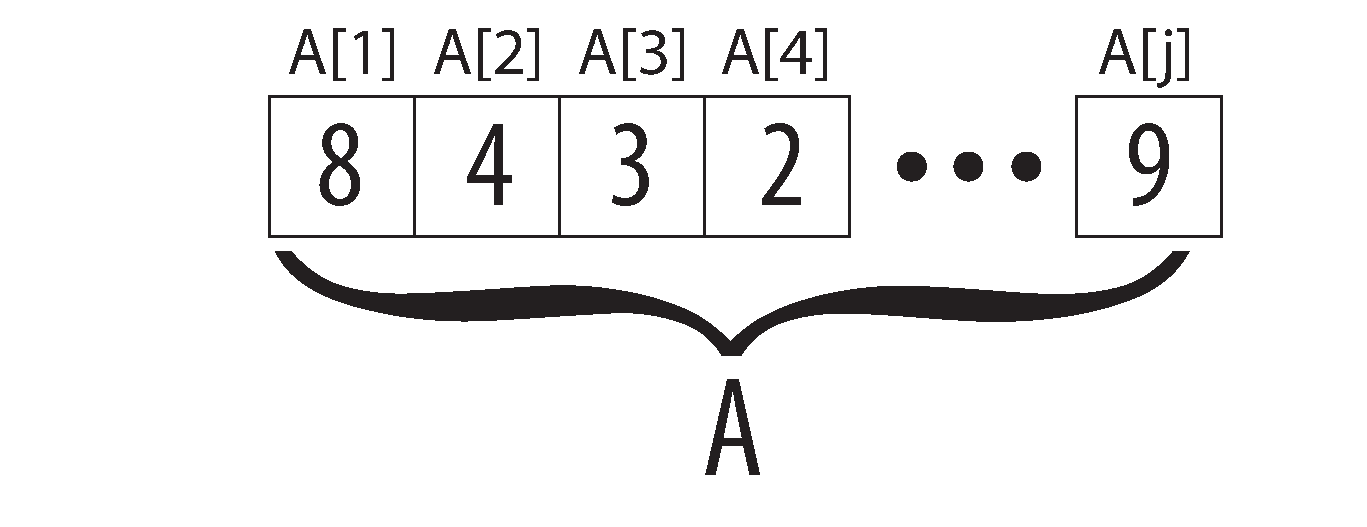
\includegraphics[scale=0.4]{fig/Array.eps}%
		\caption{Illustrasi Array}%
		\label{fig:illustrasiArray}%
	\end{figure}

\begin{Petunjuk}
\label{Ptk:Array}
	\textbf{Penggunaan array}\\
	$A[i] \rightarrow$ Mengakses lokasi ke $i$ dari array yang bernama $A$.\\
	$A[4] \rightarrow$ Mengakses lokasi ke $4$ dari array yang bernama $A$.\\
	$A[i..j] \rightarrow$ Menandakan kumpulan isi array $A$ yang terdiri dari elemen $A[1],\ A[2],\ A[3],\ \ldots,\ A[j]$.\\
	$A[4] = 5 \rightarrow$ Memasukkan nilai 5 ke lokasi ke 4 dari array $A$.\\
	$b = A[4] \rightarrow$ Memasukkan nilai lokasi ke 4 dari array $A$ ke variabel $b$. \\
	$A.length \rightarrow$ Menandakan besar/panjang dari array $A$. \\
\end{Petunjuk}

		\marginnote[-4cm]{Catatan : Ilustrasi pada petunjuk \ref{Ptk:Array}, hanya menampilkan array 1 dimensi. Seiring dengan meningkatnya pembahasan, akan dikenalkan pada array berdimensi lebih dari satu !}
	
Petunjuk \ref{Ptk:Array} beberapa kali menyebutkan istilah \textbf{lokasi}. Pada algoritma ataupun pemrograman, ini lebih dikenal dengan dengan indeks. Walaupun pada gambar \ref{fig:illustrasiArray}, indeks dimulai dari 1(satu), perlu diketahui bahwa pada kebanyakan bahasa pemrograman, termasuk python, indeks pada array selalu dimulai dari 0 dan berakhir pada (panjang data-1). \\

Perhatikan bahwa contoh \ref{Ptk:Array} diatas, sebuah \textit{statement} tunggal hanya mewakili satu nilai dari sekian banyak data yang ada di dalam array. $A[4]$ misalnya, hanya mengakses indeks ke-4 dari data A. Pertanyaannya adalah bagaimana jika kita memerlukan perhitungan jumlah total dari untuk seluruh data pada array yang berisi bilangan bulat ? Disinilah peran dari struktur \textit{Repetition/Looping}(Perulangan). Agar lebih mengerti mengenai hubungan perulangan dan array, perhatikan contoh berikut ini : 
\pagebreak
 \begin{contoh}
	\textbf{ Jumlah Total Pada Array I}
\begin{listprog}{JumlahTotalArray.py}
\label{lst:JumlahTotalArray}
\begin{lstlisting}[language=Python]
	kumpulanBilangan = [10,20,30,40,50,60,70,80,90,100]
	jumlah = 0
	for i in range(len(kumpulanBilangan)):
		print(kumpulanBilangan[i])
		jumlah += kumpulanBilangan[i]
	print(jumlah)	
\end{lstlisting}
\end{listprog}
\end{contoh}

Contoh \ref{lst:JumlahTotalArray} diatas dibuat sedemikan rupa untuk menunjukkan adanya akses terhadap indeks dari array. Terdapat alternatif lain pengaksesan array melalui looping yang ditunjukkan melalui Contoh \ref{lst:JumlahTotalArray2} berikut : 

 \begin{contoh}
	\textbf{Jumlah Total Pada Isi Array II}
\begin{listprog}{JumlahTotalArray2.py}
\label{lst:JumlahTotalArray2}
\begin{lstlisting}[language=Python]
	kumpulanBilangan = [10,20,30,40,50,60,70,80,90,100]
	jumlah = 0
	for bilangan in kumpulanBilangan:
		print(bilangan)
		jumlah += bilangan
	print(jumlah)	
\end{lstlisting}
\end{listprog}
\end{contoh}

Perhatikan beda contoh \ref{lst:JumlahTotalArray} dan \ref{lst:JumlahTotalArray2}, Pada contoh \ref{lst:JumlahTotalArray} akses bilangan dilakukan dengan akses indeks, sedangkan \ref{lst:JumlahTotalArray2} akses bilangan langsung dilakukan tetapi tanpa akses indeks. Walau tanpa akses indeks, keduanya harus tetap melibatkan struktur perulangan.\\
Sama seperti array bertipe data-lain, Sebuah \textit{String} sebenarnya sudah merupakan array dari karakter. Secara algoritma, Anda dapat mengakses karakter-karakter dari \textit{String}. Perhatikan proses akses array karakter berikut pada algoritma membalikkan kata : 

\begin{contoh}
	\textbf{Membalikkan Kata (\textit{for})}
\begin{listprog}{BalikKata.py}
\label{lst:BalikKata}
\begin{lstlisting}[language=Python]
	kata = ``Mahasiswa``
	
	#start : panjang kata mahasiswa -1 
	#        (indeks terakhir)
	#stop	: berhenti pada saat sudah -1
	#dari start ke stop dengan step : -1
	for i in range(len(kata)-1, -1, -1):
		print(kata[i])
\end{lstlisting}
\end{listprog}
\end{contoh}

\begin{contoh}
	\textbf{Membalikkan Kata (\textit{while})}
\begin{listprog}{BalikKata2.py}
\label{lst:BalikKata2}
\begin{lstlisting}[language=Python]
	kata = ``Mahasiswa``
	indeks = len(kata) - 1
	while(indeks>=0):
		print(kata[indeks])
		indeks -= 1
	\end{lstlisting}
\end{listprog}
\end{contoh}


\FloatBarrier
\subsection{Perulangan Bersarang}
Sebuah perulangan dapat memiliki perulangan di dalamnya dan perulangan yang di dalam tersebut juga dapat juga dapat memiliki perulangan lainnya di dalam. Perulangan yang di dalam tersebut tidaklah harus menggunakan \textit{statement} yang sama dengan perulangan induknya. Misalnya, boleh saja kita menggunakan \textit{statement} perulangan \textit{for} di dalam \textit{statement} perulangan \textit{while} dan juga sebaliknya. Algoritma berikut akan menunjukkan salah satu struktur perulangan bersarang. Ini merupakan salah satu dari kombinasi struktur dasar pada algoritma. \\

Implementasi Perulangan Bersarang dapat dijumpai pada beberapa permasalahan sebagai berikut : 
\begin{itemize}
	\item Ketika akan membandingkan kecocokan dua buah array yang tidak tidak terurut. 
	\item Proses pengurutan 
	\item Mencetak deret bilangan prima dari dari 0 sampai $N$
	\item Proses perhitungan yang melibatkan array berdimensi lebih dari 1, misalnya matriks
	\item Berbagai permasalahan lain yang membutuhkan perulangan bersarang
\end{itemize}

Perhatikan Contoh \ref{cth:angkaBertingkat1} dan \ref{cth:angkaBertingkat2} berikut yang menunjukkan penggunaan perulangan bersarang untuk mencetak bilangan secara bertingkat. 

\begin{contoh}
	\textbf{Bilangan Bertingkat (\textit{for})}
	\label{cth:angkaBertingkat1}
\begin{listprog}{AngkaBertingkat.py}
\label{lst:angkaBertingkat}
\begin{lstlisting}[language=Python]
	for i in range(5):
			for j in range(i+1):
					print(j, end=' ')
			print()
	\end{lstlisting}
\end{listprog}
\end{contoh}

\begin{contoh}
	\textbf{Bilangan Bertingkat (\textit{while})}
	\label{cth:angkaBertingkat2}
\begin{listprog}{AngkaBertingkat2.py}
\label{lst:angkaBertingkat2}
\begin{lstlisting}[language=Python]
	i=0
	while(i<=4):
			j=0    
			while(j<=i):
					print(j, end=' ')
					j += 1
			print()
			i += 1
	\end{lstlisting}
\end{listprog}
\end{contoh}

Perhatikan bahwa sudah dijelaskan sebelumnya bahwa perulangan bersarang tidak wajib merupakan menggunaka \textit{statement} perulangan yang sama.

\begin{contoh}
	\textbf{Bilangan Bertingkat (\textit{while})}
	\label{cth:angkaBertingkat3}
\begin{listprog}{AngkaBertingkat3.py}
\label{lst:angkaBertingkat3}
\begin{lstlisting}[language=Python]
	i=0
	while (i<=4):
			for j in range(i+1):
					print(j, end=' ')
			print()
			i += 1
	\end{lstlisting}
\end{listprog}
\end{contoh}

\marginnote{Dapatkah Anda membuat kombinasi \textit{for} dan \textit{while} nya ?}


Agar mahir pada Implementasi perulangan lanjut, latihan sangat dibutuhkan. Maka, pembahasan akan lebih banyak akan dijelaskan dalam bentuk permasalahan - permasalahan pada latihan dan praktek. 

\section{Latihan : Perulangan}

\begin{pemrograman}
Lakukan perumusan masalah, pembuatan algoritma \& program untuk membuat Urutan dan Deret sebagai berikut : 
\begin{enumerate}
	\item 1 + 2 + 3 + 4 + 5 + 6 + 7 ...  = HASIL
	\item 2 + 4 + 6 + 8 + 10 + 12 + 14 ...  = HASIL
	\item 3 + -5 + 7 + -9 + 11 + -13 + 15 ... = HASIL
	\item 1/2 + 2/3 + 3/4 + 4/5 + 5/6 + 7/8 + ...  = HASIL
	\item -2/1 + 4/3 + -6/5 + 8/7 + -10/9 + 12/11 + ...  = HASIL
\end{enumerate}
\end{pemrograman}

\begin{pemrograman}
Lakukan perumusan masalah, pembuatan algoritma \& program untuk mengkonversi bilangan Desimal ke Biner dan Biner ke Desimal
\end{pemrograman}

\begin{pemrograman}
Sediakan sebuah Array yang memiliki 100 buah angka acak. Lakukan perhitungan terhadap : 
\begin{enumerate}
	\item Rata-Rata
	\item Standar Deviasi
\end{enumerate}
\end{pemrograman}

\begin{pemrograman}
Lakukan proses enkripsi sederhana terhadap kata menjadi angka - angka sesuai urutan abjad dengan melakukan proses pembalikkan kata terlebih dahulu. Misalkan kata ``MAHA``, lakukan langkah - langkah berikut :
\begin{enumerate}
	\item 1. Balikkan Kata Menjadi ``AHAM``
	\item 2. Ubah menjadi angka dengan hasil ``1 8 1 13``
\end{enumerate}
\end{pemrograman}



\begin{pemrograman}
Untuk setiap input N lakukan pencetakan terhadap pola sebagai berikut: (Contoh N = 5)
\begin{itemize}
	\item POLA 1 \\
				* \\
				** \\
				*** \\
				**** \\
				***** \\
	\item POLA 2 \\
				***** \\
				**** \\
				*** \\
				** \\
				* \\
	\item POLA 3 \\
				***** \\
				***** \\
				***** \\
				***** \\
				***** \\
	\item POLA 4 \\
				54321 \\
				5432 \\
				543 \\
				54 \\
				5 \\
		\item POLA 5 \\
			1 \\
			12 \\
			123 \\
			12345 \\
			1234 \\
			123 \\
			12 \\
			1 \\
\end{itemize}
\end{pemrograman}

\begin{pemrograman}
Cetak pola berukuran 5x10 berikut ini !
OXOXOXOXOX\\
OXOXOXOXOX\\
OXOXOXOXOX\\
OXOXOXOXOX\\
OXOXOXOXOX\\
OXOXOXOXOX\\
OXOXOXOXOX\\
OXOXOXOXOX\\
OXOXOXOXOX\\
OXOXOXOXOX\\
Catatan: Lakukan tanpa melibatkan struktur percabangan !
\end{pemrograman}

\begin{pemrograman}
Untuk setiap kata yang diinput lakukan pencetakan kata tersebut secara diagonal \\
M \\
~I \\
~~K \\
~~~R \\
~~~~O \\
~~~~~S \\
~~~~~~K \\
~~~~~~~I \\
~~~~~~~~L \\
\end{pemrograman}


\begin{pemrograman}
Untuk setiap kata yang diinput, lakukan pencetakan terhadap alfabet yang ada dalam kata tersebut (tidak harus berurutan)  \\
Misal : Kata = ``pertemanan``
p e r t m a n \\
\end{pemrograman}


	
 
